\documentclass[t]{beamer}
%%\usetheme{Szeged}
\usetheme{Antibes}
\usecolortheme{dolphin}
\usepackage{cmap}					%поиск в pdf
\usepackage[T2A]{fontenc}			% кодировка
\usepackage[utf8]{inputenc}			% кодировка исходного текста
\usepackage[english,russian]{babel}	% локализация и переносы
%%% Работа с картинками
\usepackage{graphicx}  % Для вставки рисунков
\graphicspath{{images/}{images2/}}  % папки с картинками
\setlength\fboxsep{3pt} % Отступ рамки \fbox{} от рисунка
\setlength\fboxrule{1pt} % Толщина линий рамки \fbox{}
\usepackage{wrapfig} % Обтекание рисунков текстом

%%% Работа с таблицами
\usepackage{array,tabularx,tabulary,booktabs} % Дополнительная работа с таблицами
\usepackage{longtable}  % Длинные таблицы
\usepackage{multirow} % Слияние строк в таблице

%%% Программирование
\usepackage{etoolbox} % логические операторы

%%% Другие пакеты
\usepackage{lastpage} % Узнать, сколько всего страниц в документе.
\usepackage{soul} % Модификаторы начертания
\usepackage{csquotes} % Еще инструменты для ссылок
%\usepackage[style=authoryear,maxcitenames=2,backend=biber,sorting=nty]{biblatex}
\usepackage{multicol} % Несколько колонок

%%% Картинки
\usepackage{tikz} % Работа с графикой
\usepackage{pgfplots}
\usepackage{pgfplotstable}

\title{Senty}
\author{Балакший Андрей \and Сухочев Александр 
	\and \newline Куратор:Юрий Курочкин}
\date{19 мая 2015}
\institute[Computer Science Center]

\begin{document}
	\frame[plain]{\titlepage}
	
	
	\section{О проекте}
	\begin{frame}
		\frametitle{\insertsection}
		\textbf{Поиск упоминаний и сентиментальная разметка коротких и 	очень коротких текстов.(с использованием "чистой" разметки обучающего множества)}
	\end{frame}
	
	
	\section{Вдохновение}
	\begin{frame}
		\frametitle{\insertsection}
		\textbf{Прочитали статью ребят из Стэнфорда о сентиментальной разметке твитов. Ребята производили "грязную" разметку твитов(разметка по смайликам) и обучались по ней.}\pause
		
		\textbf{Захотелось чего-то аналогичного, но с русским языком и с "чистой" разметкой(разметкой вручную).}
	\end{frame}
	
	
	\section{Цель}
	\begin{frame}
		\frametitle{\insertsection}
		\textbf{Хотим по короткому тексту понимать настроение человека, написавшего его.}
	\end{frame}
	
	
	\section{Что хотим сделать}
	\begin{frame}
		\frametitle{\insertsection}
		\begin{itemize}
			\item Найти источник для обучения, содержащий высказывания людей по разным темам.	
			\item Придумать различные фичи для текстов из нашего источника(признаки, которые помогут определять настроения людей, написавших данный текст) и реализовать по ним машинное обучение.
		\end{itemize}
	\end{frame}
	
	
	\section{Этапы выполнения}
	\subsection{Получение материала для обучения}
	\begin{frame}
		\frametitle{\insertsection}
		\framesubtitle{\insertsubsection}
		\textbf{Необходимо получить материалы для обучения.}\pause
		
		\textbf{Решение: \newline Парсим цитаты с bash.im с помощью Beautiful Soup и сохраняем их в формате json.}
		
\includegraphics[scale = 0.8]{images/bash_im.png}
		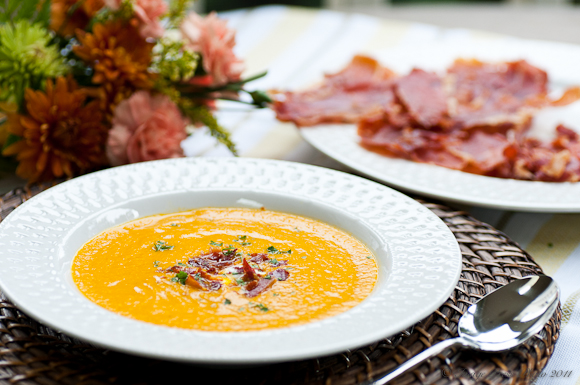
\includegraphics[scale = 0.3]{images/beautiful_soup.jpg}
	\end{frame}
	
	
	\subsection{Фичи}
	\begin{frame}
		\frametitle{\insertsection}
		\framesubtitle{\insertsubsection}
		\textbf{Фичи представляют собой дополнительные опции экстрактора. Их можно использовать в различных комбинациях для достижения высокой точности машинного обучения.}
	\end{frame}
	
	
\end{document}